\documentclass{article}
\usepackage{tikz}
\usetikzlibrary{arrows.meta, positioning}

\begin{document}

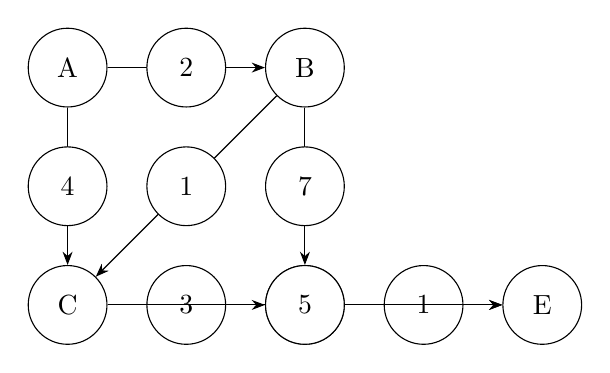
\begin{tikzpicture}[
    ->, 
    >=Stealth,
    node distance=2cm and 2cm,
    every node/.style={circle, draw, minimum size=1cm},
    edge label/.style={midway, fill=white, inner sep=2pt}
]

% Nodes
\node (A) {A};
\node (B) [right=of A] {B};
\node (C) [below=of A] {C};
\node (D) [below=of B] {D};
\node (E) [right=of D] {E};

% Edges with weights
\draw (A) -- (B) node[edge label] {2};
\draw (A) -- (C) node[edge label] {4};
\draw (B) -- (C) node[edge label] {1};
\draw (B) -- (D) node[edge label] {7};
\draw (C) -- (D) node[edge label] {3};
\draw (D) -- (E) node[edge label] {1};
\draw (C) -- (E) node[edge label] {5};

\end{tikzpicture}

\end{document}